\chapter{Trabalhos relacionados}

A utilização de ferramentas de inteligência artificial para diagnósticos em equipamentos tem se destacado como uma solução promissora no contexto da manutenção preventiva, especialmente diante do aumento da complexidade dos sistemas industriais e da necessidade de maior confiabilidade operacional \cite{Salvi2021}. O avanço tecnológico e a crescente disponibilidade de dados impulsionaram o desenvolvimento de métodos automatizados, tornando o diagnóstico mais eficiente e preciso.

No setor elétrico, particularmente no sistema elétrico de potência, essas soluções têm ganhado relevância devido à criticidade dos ativos e ao impacto direto na continuidade do fornecimento de energia. A detecção precoce de falhas em componentes como isoladores, transformadores e linhas de transmissão é fundamental para evitar interrupções e reduzir custos de manutenção \cite{wang2023}. O uso de inteligência artificial permite analisar grandes volumes de dados e identificar padrões complexos, superando limitações das abordagens tradicionais.

Diante desse cenário, diversos pesquisadores têm buscado aprimorar os métodos de diagnóstico automatizado, propondo novas técnicas e avaliando o impacto de diferentes estratégias de processamento de imagens e aprendizado profundo. As próximas seções apresentam uma revisão dos principais trabalhos relacionados, com o objetivo de contextualizar a importância do tema e caracterizar o estado da arte na área.

\section{Análise Sustentável da Detecção de Falhas em Isoladores Baseada em Otimização Visual Refinada}
O primeiro estudo aborda a detecção de falhas em isoladores em linhas de transmissão aéreas, destacando a vulnerabilidade desses componentes a fatores ambientais. A inspeção manual é ineficaz devido ao alto volume de dados e à complexidade dos fundos das imagens, levando à aplicação da rede neural convolucional de atenção regressiva (RA-CNN). O método proposto melhora a acurácia da detecção ao empregar extração de características em múltiplas escalas e operações recursivas, com otimização pelo algoritmo de Enxame de Partículas (PSO). Os resultados indicam que a RA-CNN (1+2+3) atinge 85,3\% de acurácia, superando os modelos FCAN e MG-CNN. Além disso, a abordagem proposta demonstra maior eficiência em tempo real, atingindo 25,4 FPS. \cite{wang2023}

\section{Detecção de Falhas em Isoladores em Imagens Aéreas de Linhas de Transmissão de Alta Voltagem Baseada em Modelo de Aprendizado Profundo}
O segundo estudo foca na detecção de falhas em isoladores por meio de imagens aéreas, utilizando um modelo YOLO modificado, denominado CSPD-YOLO, baseado no YOLO-v3 e na Rede Parcial de Estágio Cruzado. A pesquisa envolve a criação do conjunto de dados 'InSF-detection', composto por 1.331 imagens e 2.104 falhas rotuladas. O modelo CSPD-YOLO se destaca por uma alta acurácia (AP = 98,18\%) e eficiência no processamento (0,011 s), superando modelos tradicionais como YOLO-v3 e YOLO-v4. A análise qualitativa indica que o método é eficaz mesmo em cenários complexos, como presença de rios, vegetação e torres de energia. \cite{liu2021}

\section{Detecção de Defeitos em Isoladores por Imagem Baseada em Processamento Morfológico e Aprendizado Profundo}
O terceiro estudo propõe um método híbrido para detecção de defeitos em isoladores, combinando aprendizado profundo (Faster RCNN) com processamento morfológico. A segmentação das imagens utiliza técnicas de transformação de forma para identificação e separação de isoladores, enquanto a detecção de falhas é realizada por um modelo matemático aplicado a imagens binárias. O Faster RCNN alcança AP = 0,9175 e \textit{recall} = 0,98, superando abordagens baseadas em ResNet, YOLO e LBP+SVM. Além disso, a análise de desempenho em diferentes níveis de voltagem e condições de ruído demonstra a robustez do modelo \cite{zhang2022}.
O processo de segmentação realizado no trabalho é apresentado na Figura \ref{fig:segmentacao_zhang2022}.

\begin{figure}[H]
    \centering
    \caption{\label{fig:segmentacao_zhang2022}Segmentação de isoladores}
    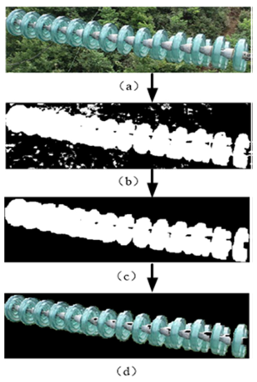
\includegraphics[width=0.6\textwidth]{img/trabalhos_relacionados/segmentacao_zhang2022.png}
    \fonte{\citeonline{zhang2022}.}
\end{figure}

\section{Comparando redes neurais convolucionais e técnicas de pré- processamento para classificação de células HEp-2 em imagens de imunofluorescência}
A pesquisa avalia seis estratégias de pré-processamento e cinco arquiteturas de CNNs de última geração para classificar células HEp-2 em imagens de imunofluorescência, uma tarefa crítica em diagnósticos médicos. Métodos como aumento de dados (rotações, espelhamentos), ajuste fino e otimização de hiperparâmetros foram testados em conjunto com arquiteturas como Inception-V3 e ResNet. Surpreendentemente, o melhor desempenho, com 98,28\% de precisão, foi alcançado ao treinar o modelo Inception-V3 do zero, utilizando apenas aumento de dados sem pré-processamento adicional. A conclusão sugere que, para esse tipo de imagem, técnicas tradicionais de pré-processamento podem ser menos impactantes quando o aumento de dados é bem implementado, desafiando a necessidade de etapas complexas de preparação. A contribuição do estudo está em mostrar que, em cenários específicos como imagens médicas de imunofluorescência, estratégias simples podem superar abordagens mais elaboradas, oferecendo uma alternativa eficiente para aplicações práticas em classificação \cite{rodrigues2020comparing}.
A Figura \ref{fig:preprocessing_rodrigues2020comparing} apresenta os métodos e combinações de pré-processamentos utilizados no trabalho.

\begin{figure}[H]
    \centering
    \caption{\label{fig:preprocessing_rodrigues2020comparing}Etapas do método proposto}
    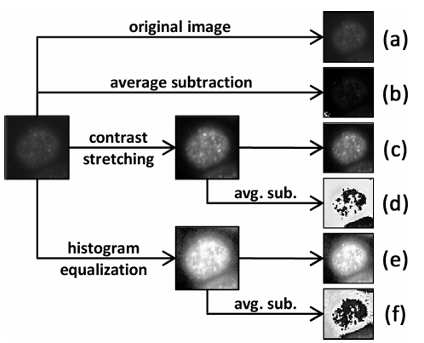
\includegraphics[width=0.6\textwidth]{img/trabalhos_relacionados/preprocessing_rodrigues2020comparing.png}
    \fonte{\citeonline{rodrigues2020comparing}.}
\end{figure}

\section{Efeitos do pré-processamento de imagens histopatológicas em redes neurais convolucionais}
O artigo analisa como diferentes níveis de pré-processamento afetam a classificação de imagens histopatológicas por CNNs, dividindo os dados em quatro categorias: imagens originais, pré-processadas normalmente (com redução de ruído e aprimoramento de células), outras pré-processadas normalmente e excessivamente pré-processadas (com operações morfológicas adicionais). Os experimentos revelam que o pré-processamento normal melhora a precisão ao remover ruídos de fundo e realçar características celulares, mas o excesso de processamento não agrega valor e pode até degradar o desempenho ao eliminar informações úteis. A conclusão enfatiza a importância de um equilíbrio no pré-processamento, recomendando ajustes moderados para maximizar a eficácia das CNNs em imagens histopatológicas. A contribuição do trabalho é fornecer uma análise comparativa detalhada que orienta pesquisadores e profissionais na escolha de técnicas de pré-processamento, evitando exageros que comprometam a qualidade dos dados em aplicações médicas \cite{ozturk2018histopathological}.

\section{O impacto de técnicas de pré-processamento e pós-processamento de imagens em frameworks de aprendizado profundo: uma revisão abrangente para análise de imagens de patologia digital}
Este trabalho explora como técnicas tradicionais de pré- e pós-processamento de imagens, como redução de ruído, correção de iluminação e segmentação, melhoram o desempenho de redes neurais em tarefas de patologia digital, incluindo classificação (tecido saudável vs. canceroso), detecção (contagem de linfócitos) e segmentação (núcleos e glândulas). Ao analisar uma ampla gama de estudos, os autores concluem que essas técnicas são indispensáveis para lidar com a variabilidade e complexidade das imagens médicas, melhorando significativamente a precisão e a robustez dos modelos de aprendizado profundo. A revisão destaca que o pós-processamento, como refinamento de contornos, também desempenha um papel crucial em tarefas de segmentação. A contribuição do artigo está em consolidar evidências sobre a eficácia dessas abordagens, oferecendo um guia abrangente para pesquisadores que buscam integrar métodos tradicionais ao treinamento de redes neurais, especialmente em contextos de patologia digital onde a qualidade dos dados é crítica \cite{Salvi2021}.

\section{Resumo dos Trabalhos}

Diversos estudos abordam o impacto do pré-processamento de imagens na análise por redes neurais convolucionais (CNNs) e outros modelos de aprendizado profundo. O estudo de \citeonline{liu2021} e \citeonline{wang2023} optam por não realizar processamentos significativos, utilizando apenas redimensionamento e normalização.

Por outro lado, \citeonline{ozturk2018histopathological} investigam diferentes algoritmos de pré-processamento, incluindo remoção de fundo, filtros de suavização e equalização de histograma, além de um método de sobre-processamento baseado em limiar adaptativo. \citeonline{rodrigues2020comparing} testam técnicas como redimensionamento, alongamento de contraste, equalização de histograma e subtração da média, constatando que o uso de imagens originais favorece o desempenho da CNN, enquanto o data augmentation tem impacto positivo. \citeonline{Salvi2021} destacam que técnicas como remoção de artefatos, normalização de cor e seleção de patches melhoram a precisão dos modelos e reduzem o tempo computacional. Por fim, \citeonline{zhang2022} exploram a segmentação de isoladores para otimizar a classificação.

\section{Justificativa da Relevância da Metodologia Proposta}

Os trabalhos analisados demonstram a importância do pré-processamento na análise de imagens, mas também indicam que determinadas abordagens podem comprometer o desempenho da CNN. Em especial, \citeonline{rodrigues2020comparing} evidenciam que a eliminação de ruídos e artefatos pode não ser sempre benéfica. Além disso, \citeonline{Salvi2021} reforçam que técnicas de segmentação e normalização podem aprimorar a análise quando aplicadas corretamente. No entanto, nenhum dos estudos analisados aborda a metodologia específica proposta nesta dissertação, o que destaca sua inovação e potencial contribuição para a área.

\section{Tabela Comparativa dos Trabalhos}

A tabela \ref{tab:comparacao_de_trabalhos_relacionados} compara os resultados de diferentes estudos sobre pré-processamento de imagens e seu impacto nos modelos de classificação de imagens. Os estudos variam desde melhorias no desempenho até riscos de sobre-processamento, destacando a falta de consenso e a necessidade de novas abordagens. A metodologia proposta neste trabalho busca preencher essa lacuna ao introduzir um método inovador para determinar os processamentos mais eficientes e otimizar os parâmetros de processamento, oferecendo uma solução mais robusta e adaptável para análise de imagens.

\begin{table}[h]
\centering
\resizebox{\textwidth}{!}{
\begin{tabular}{|l|p{11cm}|}
\hline
\textbf{Trabalho} & \textbf{Resultado do pré-processamento} \\
\hline
\citeonline{liu2021} & Sem impacto significativo \\
\hline
\citeonline{ozturk2018histopathological} & Melhorou contraste, mas risco de sobre-processamento \\
\hline
\citeonline{rodrigues2020comparing} & Afetou negativamente a CNN; data augmentation foi positivo \\
\hline
\citeonline{Salvi2021} & Melhorou precisão e reduziu tempo computacional \\
\hline
\citeonline{wang2023} & Sem impacto significativo \\
\hline
\citeonline{zhang2022} & Melhorou o desempenho do modelo \\
\hline
\end{tabular}
}
\caption{Comparação dos trabalhos relacionados}
\label{tab:comparacao_de_trabalhos_relacionados}
\end{table}

A análise desses estudos reforça a lacuna existente na literatura e a necessidade de uma nova abordagem, como a metodologia proposta nesta dissertação.
A proposta de um método para determinar os processamentos mais eficientes e otimizar os parâmetros de processamento representa uma contribuição significativa para a área de análise de imagens. Através da combinação de técnicas de pré-processamento adaptativo e otimização de parâmetros, o trabalho busca não apenas melhorar o desempenho dos modelos de aprendizado profundo, mas também oferecer uma solução prática e eficiente para cenários complexos. Essa abordagem pode impactar positivamente diversas áreas, como diagnóstico médico, inspeção industrial e análise de imagens aéreas, ao proporcionar resultados mais precisos e confiáveis. Além disso, a metodologia proposta pode servir como base para futuras pesquisas e aplicações em diferentes contextos, ampliando as possibilidades de utilização das redes neurais em tarefas desafiadoras de classificação e detecção de objetos em imagens.

\section{Considerações finais do capítulo}

A metodologia apresentada neste trabalho se diferencia dos estudos revisados ao introduzir um novo enfoque que não foi explorado anteriormente. Enquanto os trabalhos existentes se concentram em construção de modelos de redes neurais e utilização de técnicas tradicionais de pré-processamento e normalização, a metodologia deste trabalho propõe a criação de um método para determinar os processamentos mais eficientes das imagens, além de um método de otimização dos parâmetros de processamento. Além disso, a pesquisa busca integrar novas abordagens que possam aprimorar a análise de dados em contextos variados, contribuindo para a evolução das técnicas de aprendizado profundo. A implementação dessas novas abordagens poderá oferecer insights valiosos para futuras investigações e aplicações práticas.